\documentclass[10pt]{article} 
\usepackage[spanish,activeacute]{babel} %idioma español
\usepackage[utf8]{inputenc}             %transforma los tildes a lenguaje latex automáticamente
\usepackage{multirow}                   %Permite cosntruir tablas en las que algunas celdas ocupan varias filas dentro de un entorno tabular con la orden \multirow, en el caso de columnas es \multicolumn  ... \multirrow{nrow}{width}[vmove]{contenido}
% nrow: número de filas a agrupar
%width: ancho de la columna
%vmove: sirve para subir o bajar el texto (opcional)
\usepackage{epsfig}                     %permite incluir gráficos eps
\usepackage{graphicx}                   %Permite incluir gráficos e imágenes
\usepackage{subfig}                     %Permite hacer subfiguras
\usepackage{amsmath}                    %Extiende el modo matemático
\usepackage{amsthm}
\usepackage{amssymb}
\usepackage{mathrsfs}
\usepackage{hyperref}
\usepackage{colortbl} %Permite agregar color a las tablas
\usepackage{epstopdf}                 %Permite utilizar imagenes en formato eps
\usepackage{float}   %permite indicar la posición de las figuras
\usepackage[left=3cm,right=3cm,top=3cm,bottom=3cm]{geometry}
\renewcommand{\baselinestretch}{1.5}
\parskip=4pt

\usepackage{fullpage}            %%
\usepackage{fancyhdr} 
\usepackage{mdframed}            %%

\setlength{\headheight}{54pt}    %%
\setlength{\headsep}{1em}        %%
\setlength{\textheight}{8.5in}  
\setlength{\footskip}{0.5in} 


\fancypagestyle{firstpage}
{
  \fancyhf{}
  \lhead{
\includegraphics[height=5em]{LogoDFI.jpg}}
  \rhead{FI3104-1 \semestre\\
         Métodos Numéricos para la Ciencia e Ingeniería\\
         Prof.: \profesor}
  \fancyfoot[C]{\thepage}
}

\pagestyle{plain}
\fancyhf{}
\fancyfoot[C]{\thepage}


\newcommand{\semestre}{2016-2}
\newcommand{\profesor}{Valentino González}



\begin{document}

\author{Sergio Leiva M.}
\title{\textbf{Informe Tarea 9}}
\date{}
\maketitle

\thispagestyle{firstpage}


\section{Introducción}

Se pidio estudiar el movimiento de planetas cercanos al sol, los cuales estan afectados por un potencial del tipo (\ref{ec_potencial}), que es una corrección a la ley de Newton. Además se debe ocupar la tecnica de \textit{Programación orientada a objetos} (OOP, por sus siglas en ingles). 

\begin{equation}
U(r)=-\dfrac{GMm}{r}+\alpha \dfrac{GMm}{r^2}
\label{ec_potencial}
\end{equation}
  
  Para integrar este problema, se pidio que se implementaran los metodos: \textit{Runge Kutta} de orden 4 y \textit{Verlet}. Con cada uno se analizó el tipo de orbita con y sin la corrección, y además la energía en función del tiempo.
  
\section{Procedimiento}

Para el caso de \textit{RK4} se usó la implementación de la tarea anterior, con los ajustes necesarios para que trabajara con objetos,y para verlet, se siguio la metodologia de verlet con velocidad, y al igual que le caso anterior se implemento usando la tecnica \textit{OOP}.

Para encontrar el perihelio se busco el punto donde la distancia al centro y la distancia de partida, fuera la maxima, lo que caracteriza al afhelio, y como ambos deben precesar de igual manera y por temas de calculo, resulto mas simple,y dado que el primer afhelio debe estar en el punto inicial tiene sentido buscar que las distancias al centro no difieran mas alla de una tolerancia. Dado que existe una precesión, existen varios puntos de perihelio, uno por cada orbita, por lo que se tomó un promedio y una desviación estandar para ello, ademas para acotar los valores, mediante el método de inspección se encontro una tolerancia a la diferencias antes dicha, para obtener 30 valores.


\section{Resultados}

Para las constante físicas del problema y condiciones iniciales se usaron los valores de la Tabla \ref{tab_const}. Las constantes se normalizaron para simplificar tanto algebra como manejo de unidades. En el caso de las condiciones iniciales se verificaron que generaran una elipse, es decir, que la energia fuera siempre negativa.  

\begin{table}[H]
\centering
\begin{tabular}{|c|c|c|c|}
\hline
Constantes & Valor & Cond. Inicial  & Valor \\
\hline
G & 1 & x & 10 \\
\hline
m & 1 & y & 0 \\
\hline
M & 1 & vx & 0 \\
\hline
$\alpha$ & $10^{-2.937}$ & vy & 0.01 \\
\hline
\end{tabular}
\caption{Cuadro de constantes, con $\alpha = 10^{-2.XXX}$ con XXX los 3 ultimos digitos del rut 18.856.937-4. Las demas constantes fueron normalizadas para simplificar la relacion entre las masas y el algebra. Las condiciones iniciales son tales que permiten orbitas "cerradas".}
\label{tab_const}
\end{table}

Podemos ver que los graficos de la figura \ref{img_energia_5} muestran la evolución de la energia en función del tiempo, donde se encuentra que ambos casos mantienen la energia a grnades rasgos. Si vemos la figura \ref{img_prec_5} podemos ver que las orbitas descritas por ambos metodos, difieren un poco visulamente, pero es por un tema de las dimensiones de los ejes, pues son bastante similares. Para el caso de la figura \ref{img_energiayprec_30} vemos como se mantiene constante la energia aun pasando varias ciclos, y la manera en que precesa.

\begin{figure}[H]
\centering
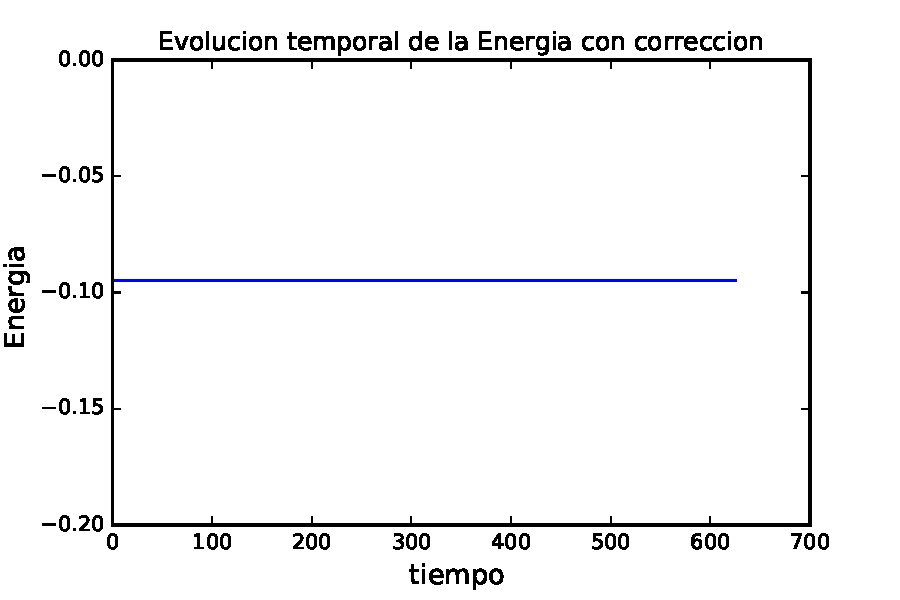
\includegraphics[scale=0.5]{energia_rk4_5.pdf}
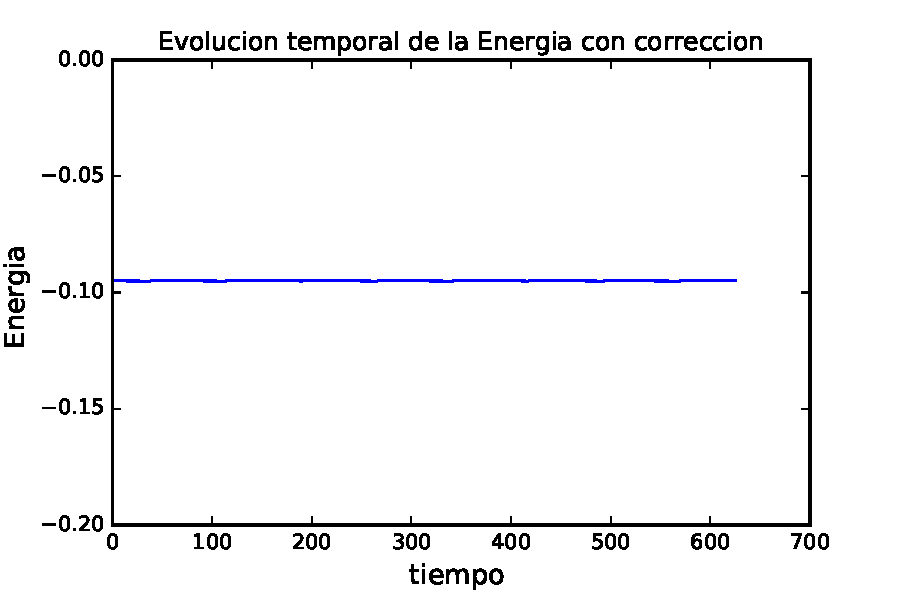
\includegraphics[scale=0.5]{energia_verlet_5.pdf}
\caption{Se muestra como en el caso de RK4 (imagen lado izq) y de Verlet (imagen lado der), no se presenta mayor diferencia en la energia. Algo que muestra una buena representación del sistema físico. Ambas imagenes son considerando solo 5 ciclos.}
\label{img_energia_5}
\end{figure}

\begin{figure}[H]
\centering
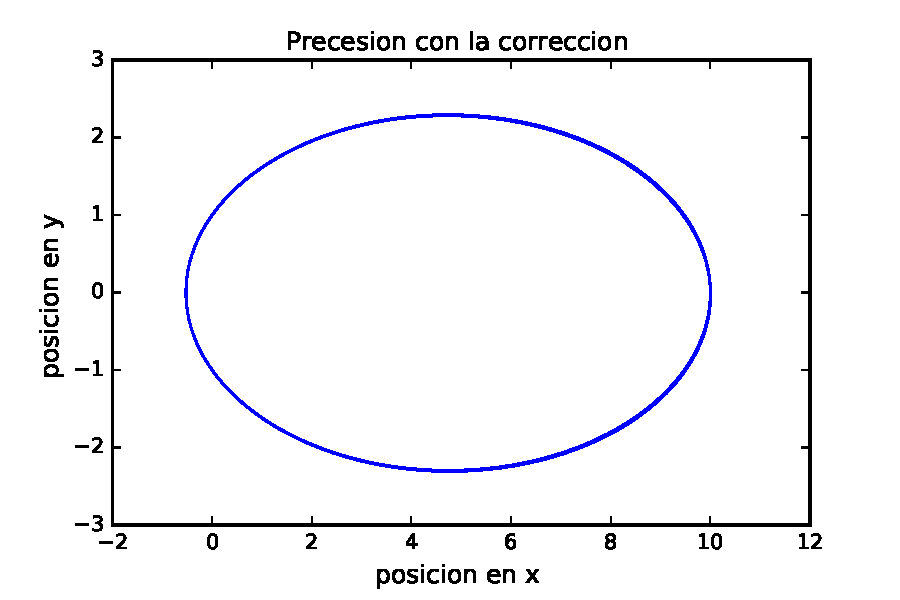
\includegraphics[scale=0.5]{pres_rk4_5.pdf}
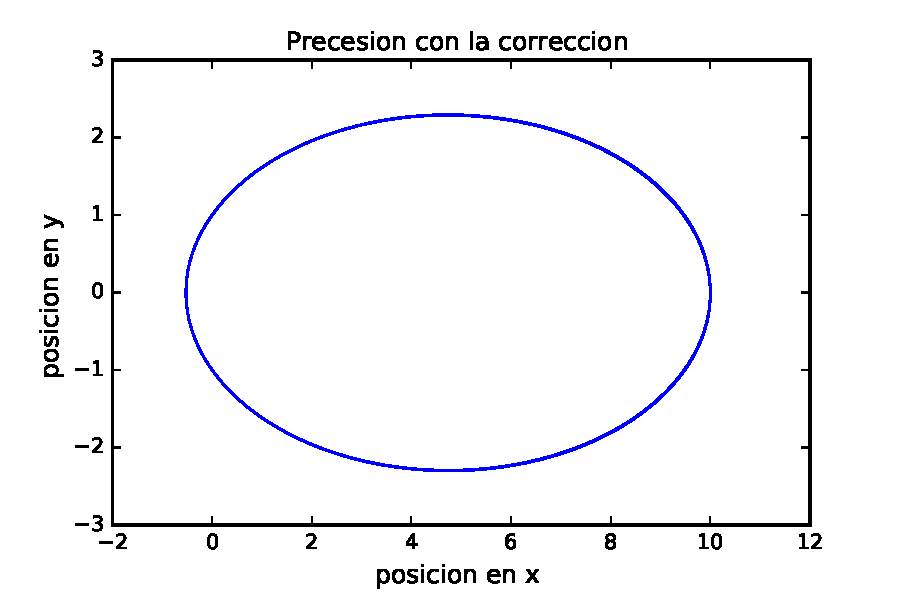
\includegraphics[scale=0.5]{pres_verlet_5.pdf}
\caption{Se muestra como en ambos casos (RK4 y Verlet) la precesión es nula, y se puede ver dado que la linea toma un color mas marcado. Ambos graficos son considerando solo 5 ciclos.}
\label{img_prec_5}
\end{figure}

\begin{figure}[H]
\centering
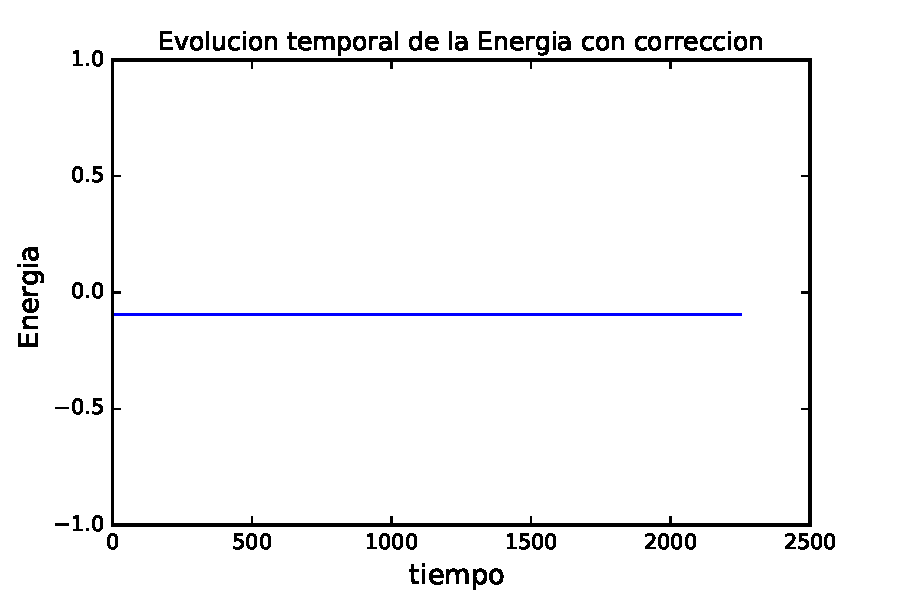
\includegraphics[scale=0.5]{energia_verlet_30.pdf}
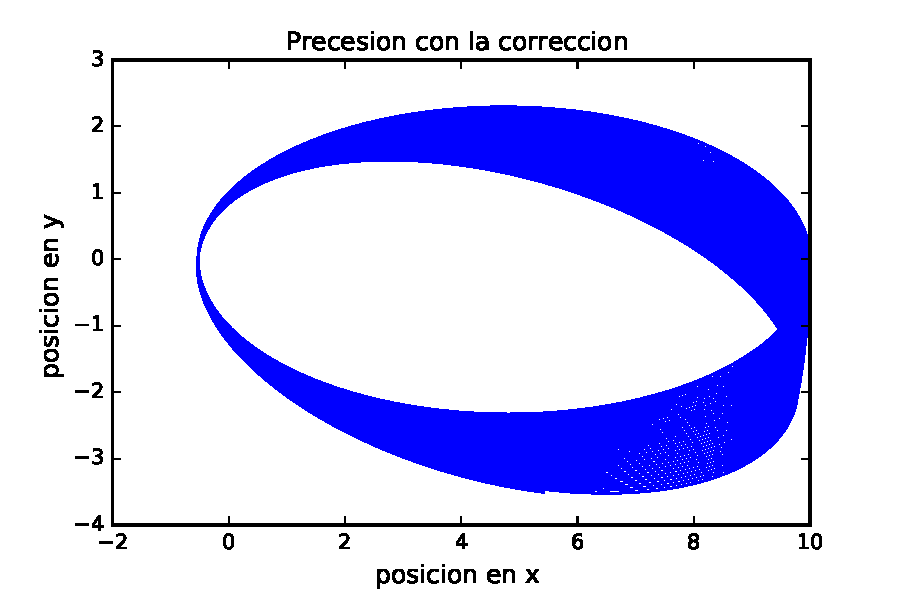
\includegraphics[scale=0.5]{pres_verlet_30.pdf}
\caption{Se muestra la precesión del planeta orbitando, se sigue con la energia constante en el tiempo pero ahora podemos ver como el perihelio comienza a variar y moverse, pero su distancia al centro no debe cambiar mucho. Ambas imagenes se graficaron con 30 ciclos.}
\label{img_energiayprec_30}
\end{figure}

\begin{table}[H]
\centering
\begin{tabular}{|c|c|c|}
\hline
Velocidad Angular & Valor & Error \\
\hline
$\omega$ & 2.4$10^{-3}$ & $\pm 7.310^{-4}$ \\
\hline
\end{tabular}
\caption{}
\label{tab_omega}
\end{table}

Para el caso de la Tabla \ref{tab_omega} podemos ver como la velocidad angular de la precesion se ve horario, pero en el grafico es antihorario, lo que viene dado que de en el cálculo, se tomo como valor antihorario positivo. 

\section{Conclusiones}
Si bien ambos algoritmos presentan buenos resultados, vemos que uno mantiene la condición de energia constante, por lo que podriamos decir que es un resultado mas real del problema. Pero no hay que dejar de lado el tema del precio que se paga por una mayor presición, como el tiempo de programación o calculo, al igual que la memoria y cantidad de datos. 


\end{document}}